\section{Graph World Model}
\label{sec:pre}

\begin{figure*}[ht]
\centering
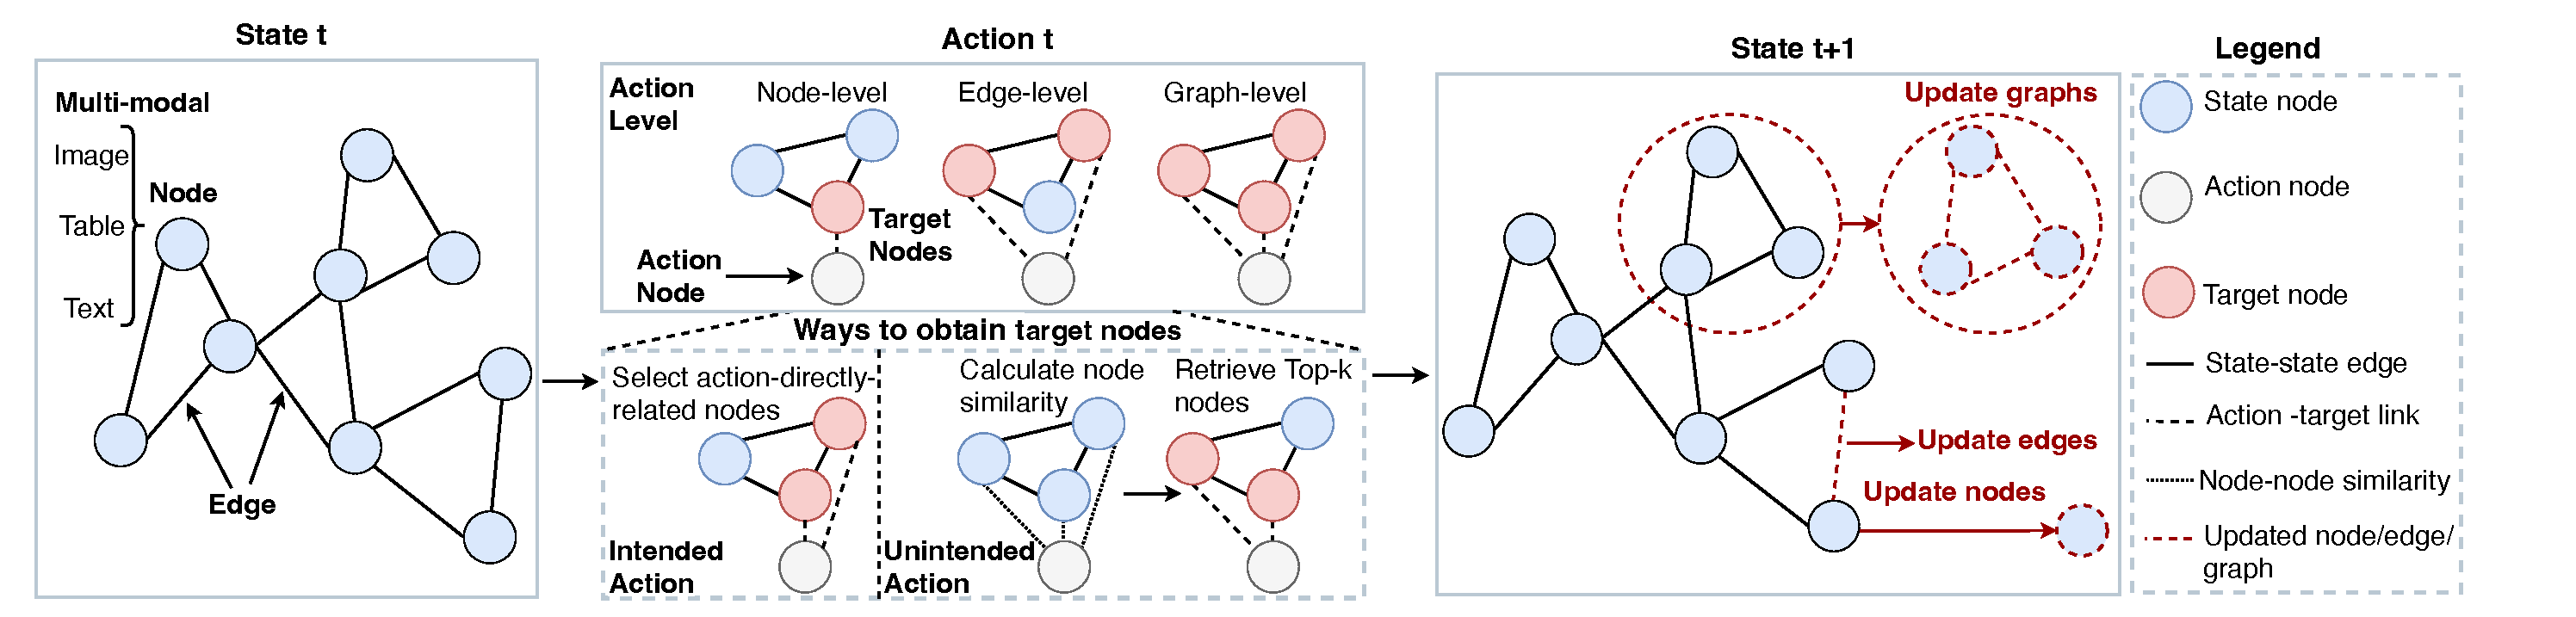
\includegraphics[width=\linewidth]{figs/r1.pdf} 
\vspace{-5mm}
\caption{\textbf{Multi-modal world state transition can be modeled via graphs}. We model the current state as a graph and each node contains one or more modalities from image, table, and text. Further, the world action is modeled as an action node that queries the current state nodes. We categorize actions into two types: intended actions, which include three levels—node, edge, and graph—and unintended actions, whose implementation involves similarity computation similar to RAG. Finally, the transition function updates states at three different levels based on state and action: update nodes, update edges, and update graphs.}
\label{fig:graph_world}
\vspace{-2mm}
\end{figure*}

\subsection{World Model Preliminaries} \label{sec:tra_wm} A world model aims to predict future states based on the current state and action, which contains the following main components: \textbf{(1) State}. The state $s$ of the world model estimates the observation of the world. It usually consists of multi-modal information and the state of the $t$ step/time slot can be depicted as $s_t$. \textbf{(2) Action}. The action $a_t$  at step/time $t$ is task-related. It can be a real-world operation, a code function in the digital world, and even some queries and instructions. \textbf{(3) Transition}. The transition $P(s_{t+1}|s_t, a_t)$ depicts the transit probability from the current state  $s_t$ to its next state $s_{t+1}$ after the execution of action $a_t$.

% \begin{itemize}[leftmargin=1em, itemsep=0pt, topsep=0pt]
%     \item \textbf{State}. The state $s$ of the world model estimates the observation of the world. It usually consists of multi-modal information and the state of the $t$ step/time slot can be depicted as $s_t$.
    
%     \item \textbf{Action}. The action $a_t$  at step/time $t$ is task-related. It can be a real-world operation, a code function in the digital world, and even some queries and instructions.
    
%     \item \textbf{Transition}. The transition $P(s_{t+1}|s_t, a_t)$ depicts the transit probability from the current state  $s_t$ to its next state $s_{t+1}$ after the execution of action $a_t$.
    
% \end{itemize} 

% \xhdr{Motivation Examples} Current world models are usually based on sequential prediction models, which utilize the sequence information of state transition but ignore the relationships among different states. As shown in Figure \ref{fig:motivation}, we take the application of the world model on individual epidemic modeling as an example. We can observe that the current world model lacks the modeling of communications among different states, which may lead to the inaccuracy of epidemic prediction or simulation. Compared with the current world model, the graph represented world model can extract the relationships among different states, which is more general and flexible in real-world applications.

% \begin{figure}[t]
% \centering
% \includegraphics[width=\linewidth]{figs/motivation.pdf} 
% \vspace{-5mm}
% \caption{\textbf{Sequence-based current world model fails in real-world individual epidemic predictions}. The left part depicts the current sequential world model on epidemic modelling, which predicts the next state only based on its previous states. The right part depicts the graph represented world model on epidemic modelling, which predicts the next state based on its previous state and the interactions (such as spatial relationships) on different visited places. Note that $p_t$ depicts the visited place at state $s_t$.}
% \label{fig:motivation}
% \end{figure}






\begin{figure*}[ht]
\centering
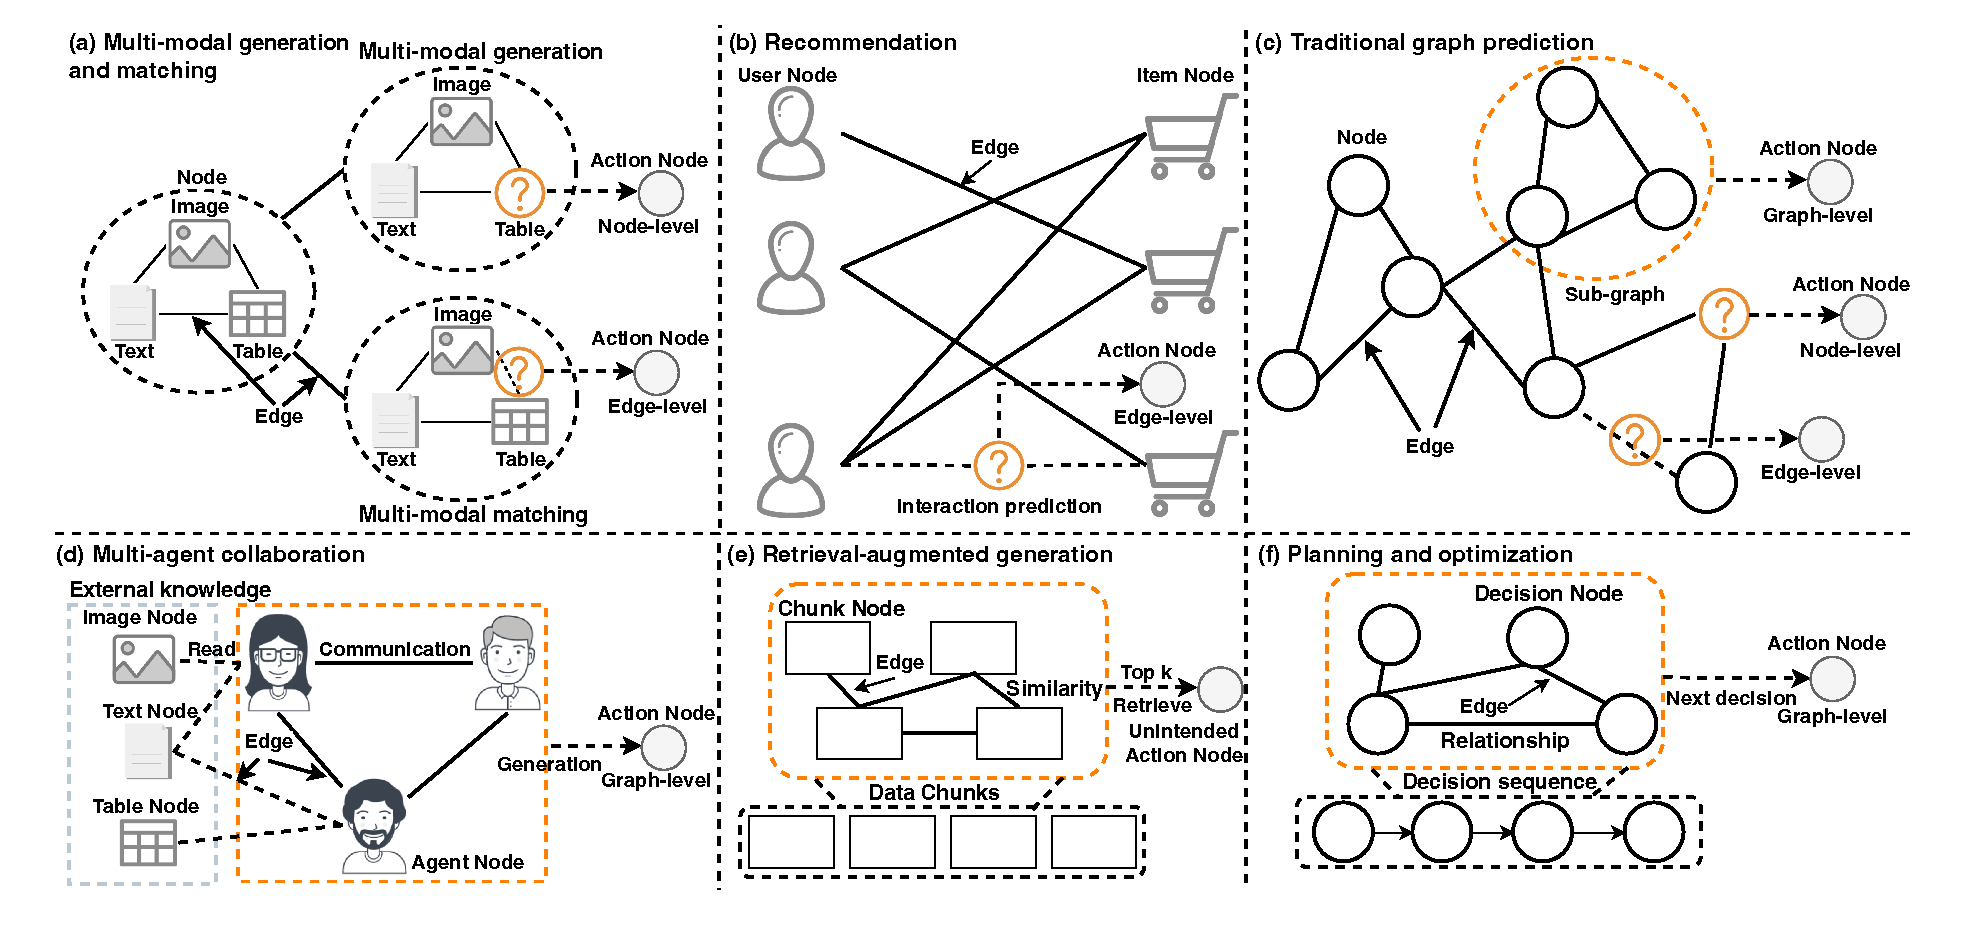
\includegraphics[width=0.95\linewidth]{figs/Instantiations.pdf} 
\vspace{-2mm}
\caption{\textbf{Instantiations of GWM}.  
(a) Multi-modal generation
and matching contains two sub-tasks. For multi-modal generation, it models modal clusters as nodes, whereas for multi-modal matching, it models nodes for each modality. It includes edges that represent inter-modal correspondences and cross-modal similarities. For these two types of subtasks, there are node-level and edge-level action nodes, respectively. (b) The state nodes of recommendation include user nodes and item nodes. Moreover, its edges are primarily derived from user-item interactions. We model edge-level action nodes to perform interaction prediction. (c) In traditional graph prediction, we follow existing work to construct task nodes and edges, and model three levels of action nodes according to different types of tasks. (d) The state nodes of multi-agent collaboration include agent nodes and multi-modal nodes from external knowledge. Its edges primarily consist of communications between agents and interactions between agents and external knowledge. We set up a graph-level action node to generate content based on the interactions of agents. (e)  Retrieval-augmented generation treats each data chunk as a state node and builds edges through the embedding similarity between chunks. For this task, we have established unintended action nodes.  (f) For planning and optimization, we model each decision as a state node and construct edges based on their relationships. We have established graph-level action nodes to generate the next decision.}
\label{fig: Instantiations of GWM}
\vspace{-3mm}
\end{figure*}

% = \mathcal{V}_a \cup \mathcal{V}_e \cup \mathcal{V}_b (a) Multi-modal generation
% and matching. (b) Recommendation. (c) Traditional graph prediction. (d)  Multi-agent collaboration. (e) Retrieval-augmented generation.  (f) Planning and optimization.}

\subsection{Multi-modal World Represented by Graphs}\label{sec:Multi-modal World} 

\xhdr{Graph for state modeling} 
% Due to the presence of multi-modal and their complex relationships in the real world, it is natural for us to model Without loss of generality, we define multi-modal state information containing images, tables, and text. 
We define the world state as a graph $ \mathcal{G} = (\mathcal{V}, \mathcal{E})$ to represent multi-modal data with complex relationships, shown in Figure \ref{fig:graph_world}. Specifically, $\mathcal{V}=\{v\}$ represents the set of nodes where each node $v=[v^a, v^b, v^e]$ consists of multi-modal information, including image $ v^a $, table $ v^b $, and text $ v^e $ modality; when a modality is absent, the corresponding tensor will be empty. $ \mathcal{E} = \mathcal{E}_p \cup \mathcal{E}_m \}$ is the edge set consists of explicit edges $ \mathcal{E}_p$ and implicit edges $\mathcal{E}_m$. Explicit edges $\mathcal{E}_p$ are often those established through expert knowledge or ground truth observations. For example, in the ogbn-arxiv dataset \citep{hu2020open}, edges are determined based on references between papers and historical collaborations between authors. Implicit edges $\mathcal{E}_m$ are those constructed through connections represented by embedding similarities in the dataset. A typical example is in many protein datasets \citep{heumos2023best,stuart2019comprehensive,stuart2019integrative}, where edges are obtained based on the similarity of certain node feature embeddings.


%% type是一种特殊attribute；之前看成type是因为node不在一个feature space; universer tokenizer; observer 

\xhdr{Different levels of world action and state transition}  We model the action $a$ as an action node that queries the current state nodes $v$ to obtain the target nodes $v_r$ using function $R$, whose process can be formulated as $v_r=R(v,a)$. We further categorize the world's actions into two types, as shown in Figure \ref{fig:graph_world}: one is directly related to the specific structures on the graph, called intended action $a_d$. It includes three levels: node-level, edge-level, and graph-level.  The other is indirectly related to the specific structures on the graph through semantic relations such as Retrieval-augmented Generation (RAG), called unintended action $a_u$. As shown in Figure \ref{fig:graph_world}, to implement this action, we can first calculate the similarity between the action node and state nodes, and then retrieve the top-k state nodes for querying.  According to the introduction in Section \ref{sec:tra_wm}, we can conclude that an action causes a transition of state $s_{t+1}=f_{tr}(s_t,a_t)$, which includes three types: update nodes, update edges, and update graphs. Here, $f_{tr}$ means a transition function, which can be a neural network.

%% action: 举例告诉它们都是 graph;给个具体例子：世界关心的entity space,简单例子：edge定义：most是implicit，不可能都表示出来，edge是某种function，存下来是否有edge，以及还有很多semantic relationship；存储state的时候，不需要一直存所有relationship，其实可以用edge function：有些function是discret function,continous function;  action是一种node，intended是明确定义，unintended是similarity function，并且很多data并一定是continuous，

%% token-level 保留了token的原有的感觉，cost太高了，insight很好；embedding space会更好; 可以参考 4*2048*4096: 命名参考llama-7b



\begin{figure*}[ht]
\centering
\vspace{-1mm}
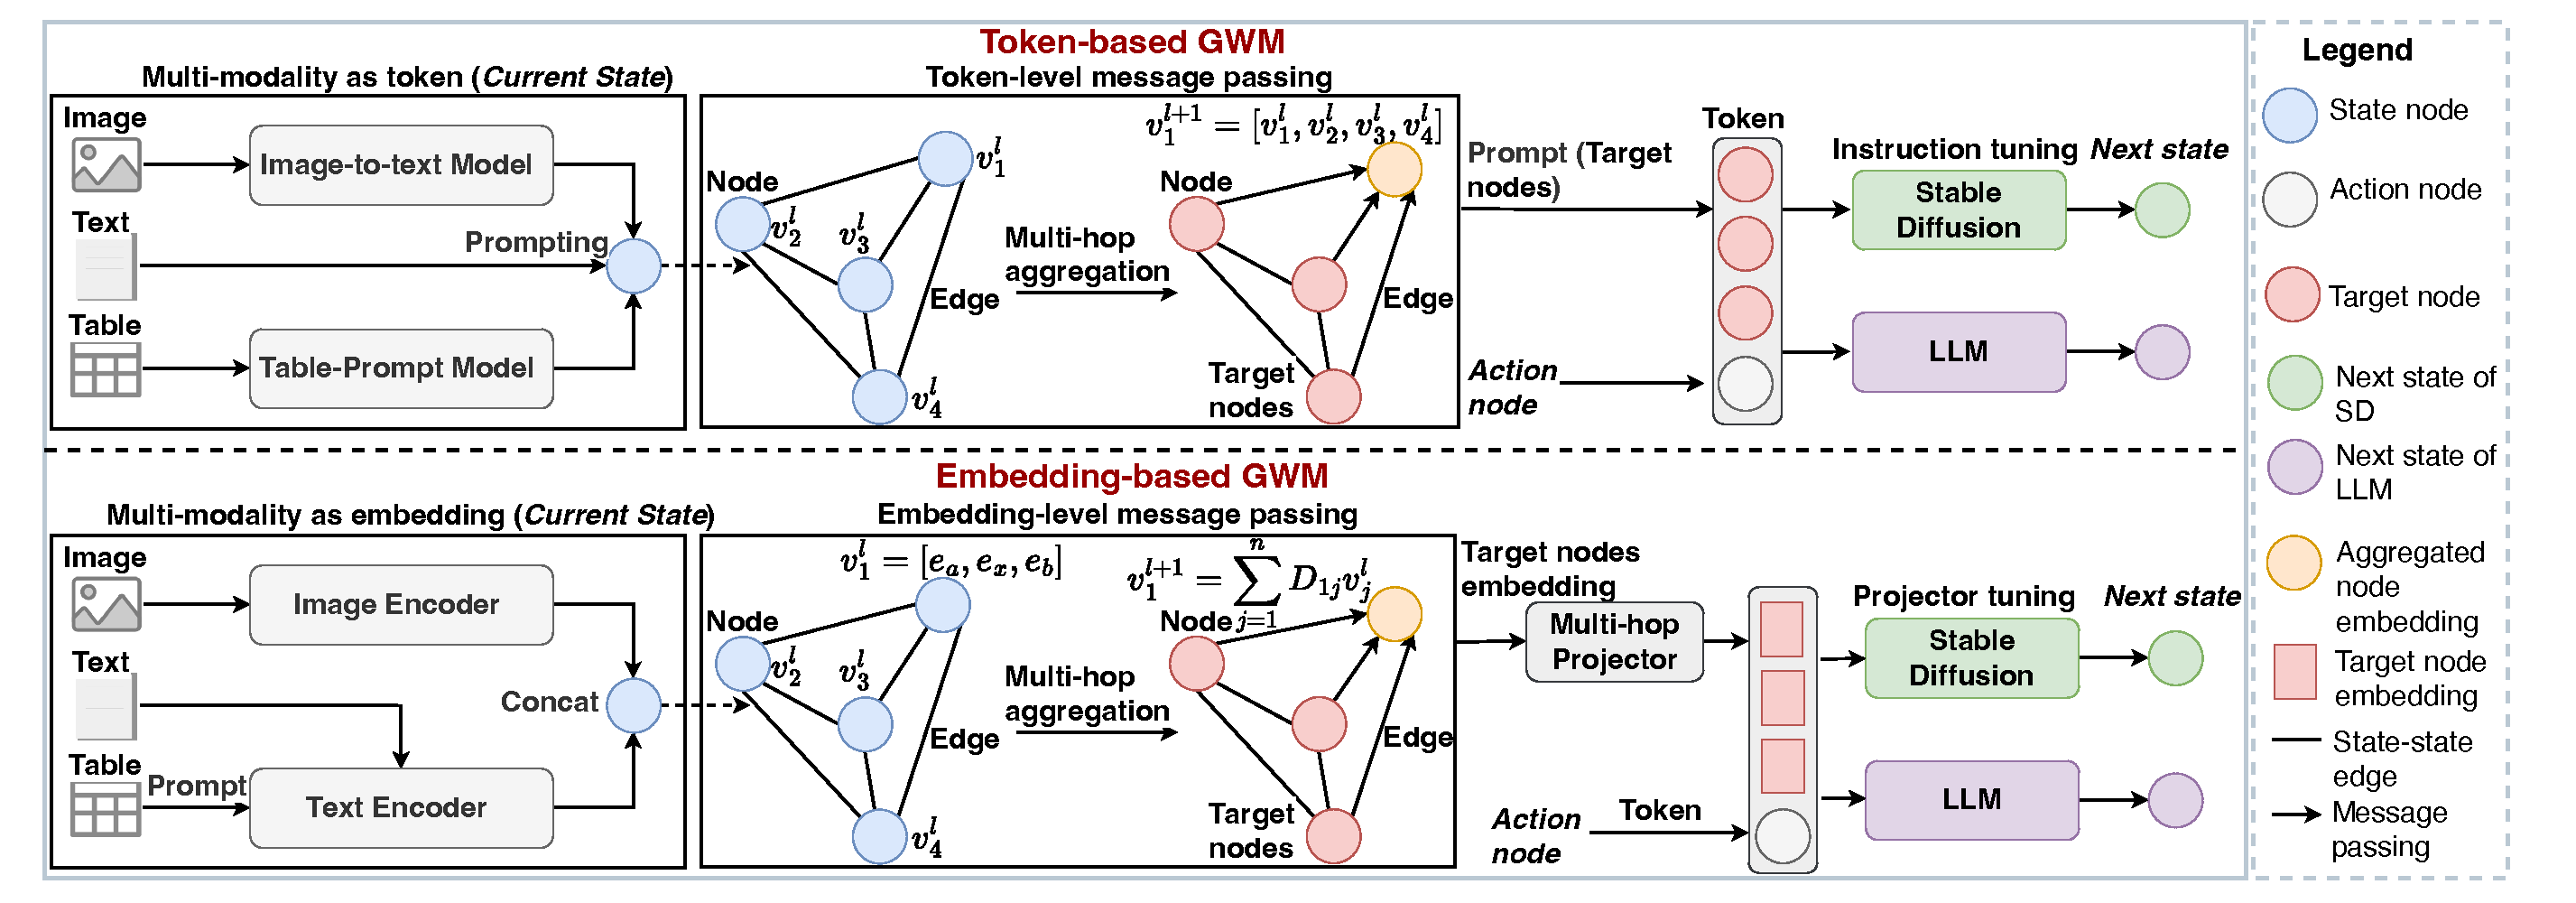
\includegraphics[width=\linewidth]{figs/r2.pdf}
\vspace{-3mm}
\caption{\textbf{Framework of GWM.} For both token-based and embedding-based GFM, we initially unify the multi-modal current state into graph nodes, conduct message passing, and then combine actions to predict the next state across different modalities through respective decoders. The key distinctions are: 1) Token-based GWM integrates multi-modalities into text, whereas embedding-based GWM uses modality-specific encoders to process them into embeddings; 2) Token-based GWM utilizes text-based methods for message passing, while embedding-based GWM operates at the embedding level; 3) Token-based GWM converts information into prompt form for the decoder, while embedding-based GWM employs a multi-hop projector to manage embedding-level information.}
\label{fig:framework}
\vspace{-4mm}
\end{figure*}



\subsection{Instantiations of GWM} \label{sec:Instantiations} 

As shown in  Figure \ref{fig: Instantiations of GWM}, we have listed some representative instantiations that can be unified into a graph world model from three aspects: (a) world prediction, (b) world generation, and (c) world optimization.

\xhdr{World prediction}
%World prediction aims to forecast and infer future states or properties based on the %distribution patterns of historical data. We have chosen three representative tasks to %illustrate how they are unified into a GWM.
\textbf{(1) Multi-modal generation and matching.} As shown in Figure \ref{fig: Instantiations of GWM}(a), the task includes two subtasks. The multi-modal generation task \citep{rombach2022high,zhang2023adding} involves predicting missing modalities given the available modal information and their interconnections. Specifically, it considers clusters of corresponding modalities (such as an image, table, and text describing the same entity) as state nodes, and the relationships between clusters, such as similarity, are treated as edges. Thus, the action node here is at the node level. The multi-modal matching task \citep{rombach2022high}, similar to CLIP's pre-training task \citep{radford2021learning}, predicts the correspondence between modalities. It treats each modality as a state node and the correspondences between modalities (including cross-modality similarity relationships) \citep{jin2024instructg2i} as edges. Here, the action node is at the edge level. \textbf{(2) Recommendation.} Recommendations \citep{ni2023content,isinkaye2015recommendation,ko2022survey} are based on the historical interactions and features of users and items to predict future interactions, as shown in Figure \ref{fig: Instantiations of GWM}(b). Specifically, it models the user nodes and item nodes as state nodes. Moreover, the action node is edge-level.
\textbf{(3) Traditional graph prediction.} Traditional graph prediction \citep{kipf2016semi,velivckovic2017graph,hamilton2017inductive} primarily focuses on three types of tasks: node-level, edge-level, and graph-level. We follow previous work's settings of nodes and edges and define the action nodes of three levels.


%As shown in the figure, we utilize the nodes and edges defined in these tasks, and according to the objectives of the tasks, there are action nodes at the node-level, edge-level, and graph-level, respectively.

\xhdr{World generation}
%World generation involves creating new, synthetic data that mimics real-world data in appearance, structure, or statistical properties. We introduce two representative tasks as follows.
\textbf{(4) Multi-agent collaboration.} As shown in Figure \ref{fig: Instantiations of GWM}(d), the purpose \citep{zhuge2024language,liu2023dynamic,wu2024agentkit} of this task is to generate task-oriented outputs based on the interaction between agents and external knowledge, as well as communication among agents. Specifically, its state nodes consist of agent nodes with different profiles, along with multi-modal nodes in external knowledge. Its edges include agent-agent and agent-knowledge relationships. The action node is graph level and the target nodes primarily include various agent nodes \citep{zhuge2024language,liu2023dynamic}.
%of discussion among agents as well as the reading relationships of agents referring to external knowledge.
%Multi-agent collaboration often results in generation based on the outcomes of agent discussions \citep{zhuge2024language,liu2023dynamic}, hence the action node is at the graph level and the target nodes primarily include various agent nodes.
\textbf{(5) Retrieval-augmented generation.} The purpose of Retrieval-Augmented Generation (RAG) is to enhance the generation capabilities of Large Language Models (LLMs) by retrieving information from external knowledge \citep{lewis2020retrieval,gao2023retrieval,zhao2024retrieval}. Recent studies such as GraphRAG \citep{edge2024local,peng2024graph} have shown that modeling the relationships between data chunks in external knowledge can enhance the generative capabilities of RAG. As illustrated in Figure \ref{fig: Instantiations of GWM}(e), we model data chunks as nodes and the similarity of embeddings between chunks as edges. As introduced in Section \ref{sec:Multi-modal World}, we design an unintended action node for RAG tasks.


\xhdr{World optimization}
\textbf{(6) Planning and optimization.} World optimization involves generating the next best decision based on a sequence of historical decisions \citep{chen2021decision,zheng2022online,siebenborn2022crucial}. Many studies have shown that modeling the relationships between historical decisions using graphs can enhance the decision-making effectiveness of world optimization \citep{jiang2018graph,munikoti2023challenges}. Following them, we model decision states as  nodes. The edges between these state nodes are often modeled based on their relationships, such as distance relationships \citep{prates2019learning} and the similarity of embeddings \citep{munikoti2023challenges, jiang2018graph}. We model the action node as the graph level.

%Such tasks aim to generate the next decision based on a sequence of historical decisions or a subset of decision points, hence we model the action node at the graph level.



% Motivated by the last section, we attempt to utilize GFM to build world model. Specifically, we have introduced how can we model the multi-modal world via graphs in Section \ref{sec:Multi-modal World}. Based on this, we introduce two different GFMs to model $f_{tr}$. Token-based GFM introduced in Sec \ref{sec:Token-based GFM} integrates the multi-modal information and various state relationships in the token level, which  is feasible but costly. Embedding-based GFM introduced in Section \ref{sec:Embedding-based GFM} extracts the multi-modal information and various state relationships in the embedding level, which is cost-friendly but causes more information losses. 







\section{Token-based GFM}\label{sec:Token-based GFM}

\subsection{Multi-modality as token} \label{sec:Multi-modal as token}

One of the easiest ways to unify multi-modalities is to transfer them into text. Specifically, as shown in Figure \ref{fig:framework}, for image nodes ${v}^a$, we utilize a pretrained image-to-text LLaVA model \citep{liu2024visual} $L$ to transform them into text nodes ${v}^{ta}=L({v}^a)$. For table nodes ${v}^b$, we employ a table-prompt model $T$ to transform them into text nodes ${v}^{tb}=T({v}^b)$ given the column names and feature values.  Specifically, each
value is paired with the corresponding column in the format
of ``\{column 1\} is \{value 1\}, \{column 2\} is \{value 2\}, ...''. Finally, we used a prompt template $P_{u}$ (specified Table \ref{prompt-template:multi-modality as token} in Appendix \ref{sec:prompt}) to unify the three modal nodes into a single text node $v_c=P_{u}({v}^{ta},{v}^{tb},v^e)$.

\subsection{Token-level message passing} 

In contrast to traditional graph message passing \citep{kipf2016semi,hamilton2017inductive,velivckovic2017graph}, we employ token-level message passing here, which aggregates the text information of neighboring nodes. Specifically, as shown in the middle part of Figure \ref{fig:framework}, for the each unified text node $v_c$, the node embeddings update of the $l$-th layer is represented as: 
\vspace{-3.5mm}
\begin{equation}
    \label{eq:sage}
    \mb{h}_v^{(l)} =f_{v}\Big(\textsc{Concat}(\mb{h}_v^{(l-1)},\{\mb{h}_u^{(l-1)}, u \in {N}(v) \})\Big),
\end{equation}
where $\mb{h}_v^{(l)}$ is the node text presentation after $l$ iterations, $\mb{h_v}^{(0)}$ has been initialized as $\mb{h_v}^{(0)}=v_c$. In addition, ${N}(v)$ denotes the direct neighbors of node $v$ and $f_{v}(\cdot)$ denotes prompting strategy functions (specified in Table \ref{prompt-template:aggregating} of Appendix \ref{sec:prompt}) to unify nodes information of different hops. 

%$\mb{h}_v^{(l)} =f_{v}\Big(\textsc{Concat}(\mb{h}_v^{(l-1)},\{\mb{h}_u^{(l-1)}, u \in {N}(v) \})\Big)$, where $\mb{h}_v^{(l)}$ is the node text presentation after $l$ iterations, $\mb{h_v}^{(0)}$ has been initialized as $\mb{h_v}^{(0)}=v_c$. In addition, ${N}(v)$ denotes the direct neighbors of $v$ and $f_{v}(\cdot)$ (prompt can be seen in Table \ref{prompt-template:aggregating} of Appendix \ref{sec:prompt}) denotes prompting strategy functions to unify nodes information of different hops. 



\subsection{Instruction tuning} \label{sec:Instruction tuning}  Based on token-level message passing, we can obtain node text representations $\mathbf{h}_v$ for each node. Combining the discussion in Section \ref{sec:Multi-modal World}, we identify the target nodes $v_r$ and their node text representations $\mathbf{h}_{vr}$, along with the action node $a$ and the state node. Further, we describe the action node using text and utilize a task-oriented prompt template $P_{sa}$ (specified in Appendix \ref{sec:prompt}) to combine the information from the target nodes and the action node, as shown in the right part of Figure \ref{fig:framework}.  In response to the different modalities in next states, we designed two types of decoders. We first designed stable diffusion (SD) to generate images.

\xhdr{Instruction tuning of SD} SD operates by performing diffusion in a compressed latent space rather than directly on pixels. Initially, the system maps an input image $x$ to a lower-dimensional latent code $\mathbf{z}=\text{Enc}(x)$ through an encoder network.
The generated latent representation $\mathbf{z}'$ is subsequently transformed back into image space via a decoder network, producing the final output $x'=\text{Dec}(\mathbf{z}')$. This latent representation $\mathbf{z}'$ is generated by the diffusion model using textual guidance from a prompt $c_T=P_{sa}(\mathbf{h}_{vr},a)$.
The fundamental optimization objective for training SD can be expressed mathematically as: 
\vspace{-1mm}
\begin{gather}
    \hspace{-1mm}\mathcal{L}=\mathbb{E}_{\mathbf{z} \sim \text{Enc}(x), c_T, \epsilon \sim \mathcal{N}(0,1), t} \left[ \|\epsilon - \epsilon_\theta(\mathbf{z}_t, t, h(c_T))\|^2 \right]
\end{gather}
During each iterative step $t$, a specialized denoising network $\epsilon_\theta(\cdot)$ estimates noise patterns by jointly processing three inputs: the current latent state $\mathbf{z}_t$, a temporal position indicator $t$, and encoded text features $h(c_T)$. The text features $h(c_T)\in\mathbf{R}^{d\times l_{c_T}}$ are extracted using CLIP's text encoder \citep{radford2021learning} $h(c_T)=\text{CLIP}(c_T)$, where $l_{c_T}$ represents the prompt length and $d$ denotes the feature dimensionality.

%$\mathcal{L}=\mathbb{E}_{\mathbf{z} \sim \text{Enc}(x), c_T, \epsilon \sim \mathcal{N}(0,1), t} \left[ \|\epsilon - \epsilon_\theta(\mathbf{z}_t, t, h(c_T))\|^2 \right]$. During each iterative step $t$, a specialized denoising network $\epsilon_\theta(\cdot)$ estimates noise patterns by jointly processing three inputs: the current latent state $\mathbf{z}_t$, a temporal position indicator $t$, and encoded text features $h(c_T)$. The text features $h(c_T)\in\mathbf{R}^{d\times l_{c_T}}$ are extracted using CLIP's text encoder \citep{radford2021learning}, where $l_{c_T}$ represents the prompt length and $d$ denotes the feature dimensionality: $h(c_T)=\text{CLIP}(c_T)$.

%\vspace{-2.5mm}
%\begin{gather}
    %\mathcal{L}=\mathbb{E}_{\mathbf{z} \sim \text{Enc}(x), c_T, \epsilon \sim \mathcal{N}(0,1), t} \left[ %\|\epsilon - \epsilon_\theta(\mathbf{z}_t, t, h(c_T))\|^2 \right],
%\end{gather}

\xhdr{Instruction tuning of LLM} We then design LLM to generate texts for both text and table modalities. We followed the standard instruction tuning practice \citep{zhang2023instruction,peng2023instruction}, which encourages LLMs to adhere to user requests when returning the outputs. For the input instruction $P_{sa}(\mathbf{h}_{vr},a)$, we supply a response representing the next predicted states, consisting of $t$ tokens and denoted as $y=\{y_1, \ldots y_t\}$. We train the LLM to yield $f_{\text{SFT}}$ via
\vspace{-1mm}
\begin{equation}\label{equ:sft}
\hspace{-1mm}\mathcal{L}_{SFT}=-\sum_{t}logP_{f_{\text{SFT}}}(y_t|P_{sa}(\mathbf{h}_{vr},a),y_1, \ldots y_{t-1}).
\end{equation}
\vspace{-7mm}


%$\mathcal{L}_{SFT}=-\sum_{t}logP_{f_{\text{SFT}}}(y_t|P_{sa}(\mathbf{h}_{vr},a),y_1, \ldots y_{t-1})$.


%\vspace{-2.5mm}
%\begin{equation}\label{equ:sft}
%\mathcal{L}_{SFT}=-\sum_{t}logP_{f_{\text{SFT}}}(y_t|P_{sa}(\mathbf{h}_{vr},a),y_1, \ldots y_{t-1}).
%\end{equation}
%\vspace{-3.5mm}

\section{Embedding-based GFM}\label{sec:Embedding-based GFM} 

Although token-based GFM can relatively simply construct a multi-modal world, it is still limited by the high token cost and a restricted multi-hop field of view. Inspired by stable diffusion, which introduces modeling in latent space rather than directly on pixels to enhance model performance and efficiency, we have introduced embedding-based GFM as shown in the bottom half of Figure \ref{fig:framework}.

\vspace{-1mm}
\subsection{Multi-modality as embedding} The embedding-based GFM unifies the multi-modal nodes in the embedding space. Firstly, as shown in Figure \ref{fig:framework}, for each modality of the node, we would assign a specific encoder. For the text modality  $ v^e$, we utilize a BERT model as the encoder $E_{b}$ to obtain its embedding $e_{t}$. As for the table node $ v^b$, we first transform it into text description as discussed in Section \ref{sec:Multi-modal as token} and then utilize a BERT model as the encoder $E_{b}$ to obtain its embedding $e_{b}$. Finally, we deploy a CLIP $E_{c}$ model to encode the image node $ v^a$ into image embedding $e_{a}$. We finally obtain the node embedding $e_v=\textsc{Concat}(e_{a},e_{t},e_{b})$ by concatenating the embeddings of all modalities involved with this node. Specifically, if a node misses some modalities, we use zero vectors for them.

%% whether to model edge



%% multi-task node一种，any task node shape: zero-hop:CLIP,二阶邻居smooth simplified GCN (pyG,SGCN:矩阵乘法，GAMLP; identiy GCN),真正的边以及implicit边，K-nearest GCN，variance; 对每个hop分别做projector； 


\subsection{Embedding-level message passing} 

In this section, we first model the relationships between nodes on the graph through multi-hop aggregation, then aggregate the information from different modalities within the nodes through cross-modal fusion into unified embeddings to pass to the subsequent decoders.

\xhdr{Multi-hop aggregation}  We designed a simplified GCN \citep{wu2019simplifying,he2020lightgcn} to implement multi-hop aggregation, which directly accomplishes parameter-free feature aggregation at the node feature level. Specifically, for the adjacency matrix $\mathcal{A}$ between nodes, we first normalize it to obtain the matrix $\mathcal{\tilde{A}}=\mathcal{D}^{-\frac{1}{2}}\mathcal{A}\mathcal{D}^{-\frac{1}{2}}$, where $\mathcal{D}$ represents the degree matrix of $\mathcal{A}$. Then, for the node vector $X_e$ composed of all node embeddings $e_v$, we use the obtained normalized adjacency matrix $\mathcal{\tilde{A}}$ to perform $l$-hop graph aggregation: $X_{e}^{(l)}=\mathcal{\tilde{A}}^{l}*X_e$, where $X_{e}^{(l)}$ is the $l$-hop graph embedding. We retain the embeddings of the first $L$ hops $[X_e,X_{e}^{(1)},\ldots,X_{e}^{(L)}]$ to the subsequent modules.  


%\begin{equation}\label{equ:zze}
%X_{e}^{(l)}=\mathcal{\tilde{A}}^{l}*X_e,
%\end{equation}
%where $X_{e}^{(l)}$ is the $l$-hop graph embedding. We retain the embeddings of the first $L$ hops $[X_e,X_{e}^{(1)},\ldots,X_{e}^{(L)}]$ to the subsequent modules.

%\begin{equation}\label{equ:zze}
%\mathcal{\tilde{A}}=\mathcal{D}^{-\frac{1}{2}}\mathcal{A}\mathcal{D}^{-\frac{1}{2}},
%\end{equation}


\xhdr{Cross-modal fusion} We further apply a parameterized projector $f_c$ to transform the multi-modalities in the node to unified embeddings: $X_{c}^{(l)}=f_c(X_{e}^{(l)})$, where $X_{c}^{(l)}$ is the unified node embedding. Specifically, we utilize a simple MLP as projector $f_c$ and output the $L$ hops embeddings $X_G=[X_c, X_{c}^{(1)}, \ldots, X_{c}^{(L)}]$ to the decoders. Note that GWM-E can be extended to heterogeneous graphs by performing separate multi-hop aggregations for each edge type, followed by flattening the resulting node embeddings into a sequence format suitable for input into the LLM decoder.

%\begin{equation}\label{equ:zze}
%X_{c}^{(l)}=f_c(X_{e}^{(l)}),
%\end{equation}
%where $X_{c}^{(l)}$ is the unified node embedding. Specifically, we utilize a simple MLP as projector $f_c$ and output the $L$ %hops embeddings $X_G=[X_c, X_{c}^{(1)}, \ldots, X_{c}^{(L)}]$ to the decoders.


\subsection{Projector tuning} \label{sec:Projector tuning}

As discussed in Section \ref{sec:Instruction tuning}, in this section we discuss the tuning of projectors for two different modalities separately.

\xhdr{Projector tuning of SD} We first incorporate graph conditioning tokens $h_G(c_G)=X_G$ into the SD models, functioning concurrently with the pre-existing text conditions $h_T(c_T)$: $h(c_T, c_G) = [h_T(c_T), h_G(c_G)] \in \mathbf{R}^{d \times (l_{c_T}+l_{c_G})}$, where $l_{c_G}$ is the length of the graph condition. The training objective then becomes:
\vspace{-1mm}
\begin{gather}
    \mathcal{L}=\mathbb{E}_{\mathbf{z} \sim \text{Enc}(x), c_T, c_G, \epsilon \sim \mathcal{N}(0,1), t} \left[ \|\epsilon - \epsilon_\theta(\mathbf{z}_t, t, h(c_T, c_G))\|^2 \right].
\end{gather}
\vspace{-6mm}

%For $h_T(c_T)$, we still use the CLIP text encoder as in the original SD.


%\begin{gather}
%    h(c_T, c_G) = [h_T(c_T), h_G(c_G)] \in \mathbf{R}^{d \times (l_{c_T}+l_{c_G})},
%\end{gather}
%where $l_{c_G}$ is the length of the graph condition. The training objective then becomes:




\xhdr{Projector tuning of LLM} We describe the action node $a$ using text as in Section \ref{sec:Instruction tuning}. We further introduce graph tokens $X_G$ into LLM.  The training objective of LLM is to maximize the probability of generating the correct next states. Combining the discussion in Section \ref{sec:Instruction tuning}, we train the LLM to yield $f_{\text{SFT}}$ via 
\vspace{-1mm}
\begin{equation}\label{eq:max}
\mathcal{L}_{SFT}=-\sum_{t}logP_{f_{\text{SFT}}}(y_t|X_G,a,y_1, \ldots y_{t-1}).
\end{equation}
We use a training approach similar to prefix tuning \citep{li2021prefix}, where we fix the LLM's parameters and only fine-tune the projector $f_c$'s parameters.


%$\mathcal{L}_{SFT}=-\sum_{t}logP_{f_{\text{SFT}}}(y_t|X_G,a,y_1, \ldots y_{t-1})$. We use a training approach similar to prefix tuning \citep{li2021prefix}, where we fix the LLM's parameters and only fine-tune the projector $f_c$'s parameters.


